\documentclass{beamer}
\usepackage[utf8]{inputenc}
\usepackage{subfig}
\usepackage{tabularx}
\usepackage{pgfpages}
\usepackage{array}
%---Propriétés presentation
\usetheme{Darmstadt}
%Pour ajouter un pied de page
\makeatletter
\setbeamertemplate{caption}[numbered]
\setbeamertemplate{footline}
{
  \leavevmode%
  \hbox{%
  \begin{beamercolorbox}[wd=.333333\paperwidth,ht=2.25ex,dp=1ex,center]{author in head/foot}%
    \usebeamerfont{author in head/foot}\insertshortauthor%~~\beamer@ifempty{\insertshortinstitute}{}{(\insertshortinstitute)}
  \end{beamercolorbox}%
  \begin{beamercolorbox}[wd=.333333\paperwidth,ht=2.25ex,dp=1ex,center]{title in head/foot}%
    \usebeamerfont{title in head/foot}\insertshorttitle
  \end{beamercolorbox}%
  \begin{beamercolorbox}[wd=.333333\paperwidth,ht=2.25ex,dp=1ex,right]{date in head/foot}%
    \usebeamerfont{date in head/foot}\insertshortdate{}\hspace*{2em}
    \insertframenumber{} / \inserttotalframenumber\hspace*{2ex} 
  \end{beamercolorbox}}%
  \vskip0pt%
}
\makeatother
%\setbeameroption{show only notes}

%setbeameroption{show notes on second screen=left}

%Slide de titre
\title{PRD 48: Soutenance Finale}
\subtitle{Magic Portrait: Améliorons la photographie de portrait}
\author{Pierre-Yves Hervo \and Paul-François Jeau}
\date{18 février 2014}

\AtBeginSection[]
{
  \begin{frame}<beamer>{}
    \tableofcontents[currentsection]
  \end{frame}
}
\begin{document}
%--------------------------------------------------------------------------------------------------------
%Garde---------------------------------------------------------------------------------------------------
%--------------------------------------------------------------------------------------------------------
\begin{frame}
    \titlepage
    \begin{center}
        \begin{figure}
		    
\includegraphics[width=0.4\textwidth]{PolytechNantes}
        \end{figure}
        \textbf{Tuteur: Matthieu Perreira Da Silva\\
	            Coordinateur: José Martinez}
	\end{center}
\end{frame}

%--------------------------------------------------------------------------------------------------------
%Plan----------------------------------------------------------------------------------------------------
%--------------------------------------------------------------------------------------------------------
\begin{frame}{Plan}
\tableofcontents
\end{frame}

%--------------------------------------------------------------------------------------------------------
%Présentation du projet----------------------------------------------------------------------------------
%--------------------------------------------------------------------------------------------------------
\section{Présentation du projet}

\subsection{Problématique et objectifs poursuivis}

\begin{frame}{Problématique et objectifs poursuivis}
\begin{itemize}
\item Projet multimédia
\item Retouche des clichés en notre possession potentiellement compliquée
\end{itemize}
\pause
\begin{block}{Problématique: }
Que traiter et de quelle manière ?
\end{block}
\pause
\begin{itemize}
\item Explorer des techniques d'améliorations des photographies de portrait
\item Proposition des nouvelles solutions possibles dans ce domaine
\end{itemize}
\end{frame}

\subsection{Points abordés lors de phase bibliographique}

\begin{frame}{Points abordés lors de phase bibliographique}
\begin{itemize}
\item Étude de critères permettant de juger l'esthétique des photographies
\item Comparaison de méthodes de correction des portraits 
\item Élaboration de deux propositions 
\end{itemize}
\end{frame}

\subsection{Planification suivie lors de la seconde phase}

\begin{frame}{Planning prévisionnel}
\begin{figure}
	\centering
		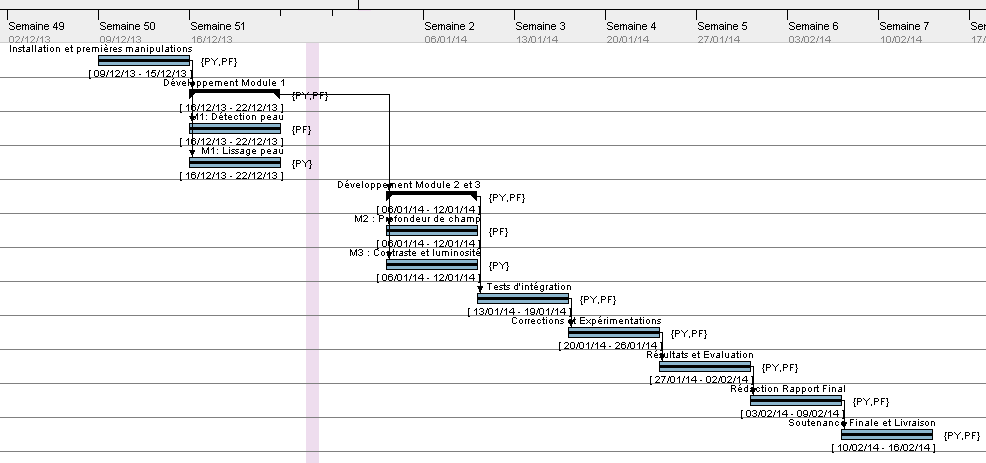
\includegraphics[width=1\textwidth]{p2_previsionnel}
	\caption{Planification prévisionnelle de la seconde phase}
	\label{fig:PlanningPrevisionnel}
\end{figure}
\end{frame}

\begin{frame}{Planning effectif}
\begin{figure}
	\centering
		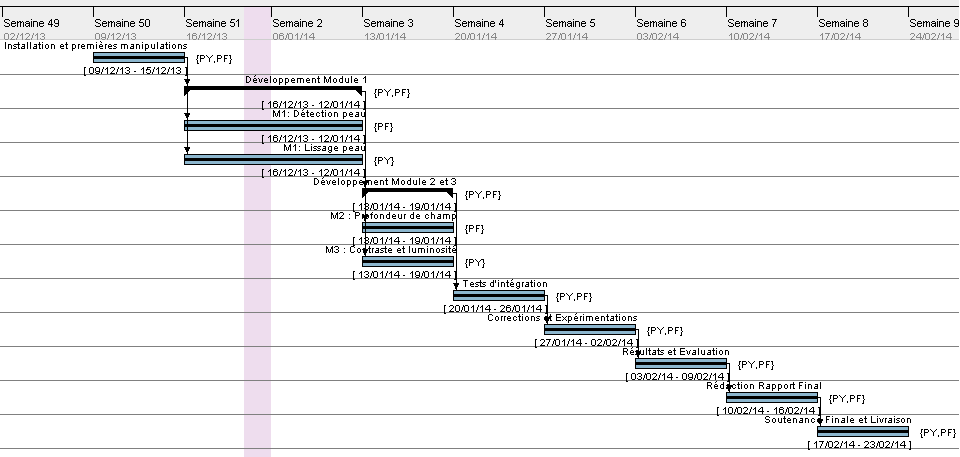
\includegraphics[width=1\textwidth]{p2_effectif}
	\caption{Planification effective}
	\label{fig:PlanningEffectif}
\end{figure}

\end{frame}
\begin{frame}{Comparaison des plannings de la seconde phase}
\begin{figure}
	\centering
		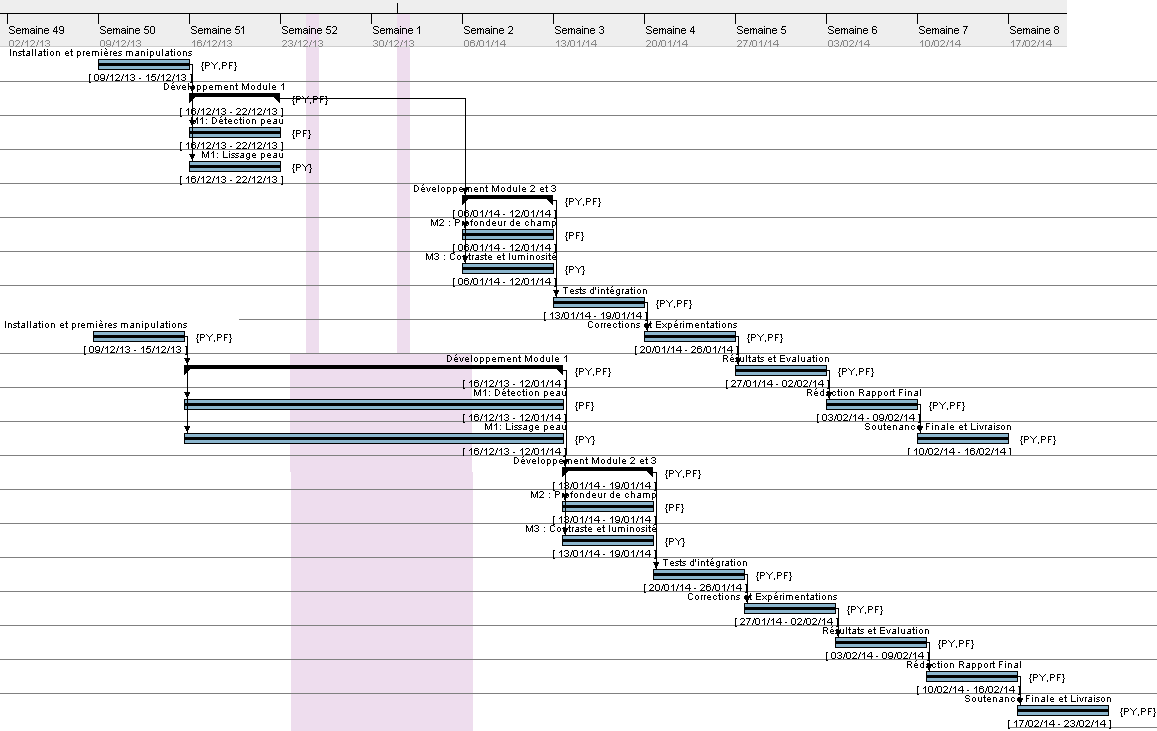
\includegraphics[width=0.95\textwidth]{p2_previ_effe}
	\caption{Comparaison des plannings de la seconde phase}
	\label{fig:PlanningEffePrevi}
\end{figure}
\end{frame}

%--------------------------------------------------------------------------------------------------------
%Proposition élue----------------------------------------------------------------------------------------
%--------------------------------------------------------------------------------------------------------
\section{Proposition élue}

\subsection{Principe de la proposition}

\begin{frame}{Principe de la proposition}
\begin{itemize}
\item Méthode basée sur le lissage de la peau et des imperfections cutanées
\item Traitement de la profondeur de champ
\item Correction du rendu final de l'image
\end{itemize}
\end{frame}

\begin{frame}{Schéma global}
\begin{figure}
\centering
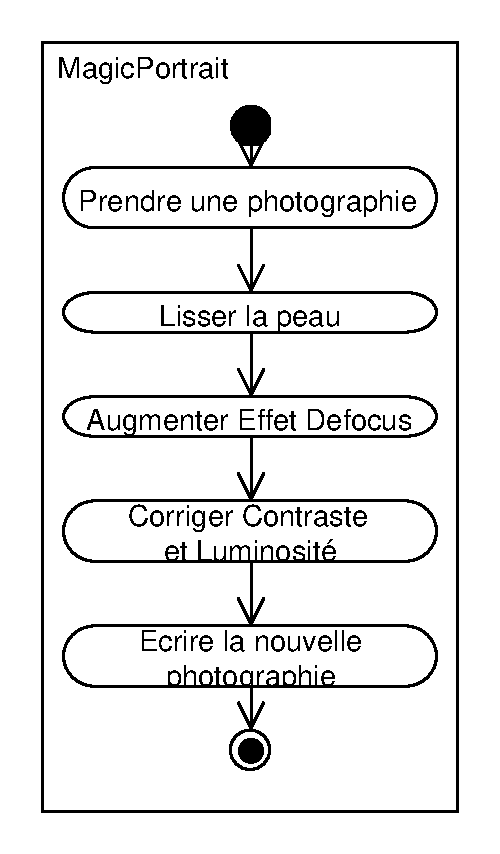
\includegraphics[width=0.35\textwidth]{DiagrammeActivites_00_Global}
\caption{Principe de fonctionnement général}
\end{figure}
\end{frame}

\subsection{Compléments bibliographiques}

\begin{frame}{Compléments bibliographiques}
\begin{itemize}
\item Méthodes de détection de la couleur peau
\item Segmentation des objets au premier plan et à l'arrière-plan
\item Manipulation et réhaussement d'histogrammes des images
\item Pour pouvoir disposer de techniques pour le développement
\end{itemize}
\end{frame}

%--------------------------------------------------------------------------------------------------------
%Développement-------------------------------------------------------------------------------------------
%--------------------------------------------------------------------------------------------------------
\section{Développement}

\subsection{Développement des modules}

\begin{frame}{Fonctionnement du module 1: Lissage de la peau}
\begin{figure}
\centering
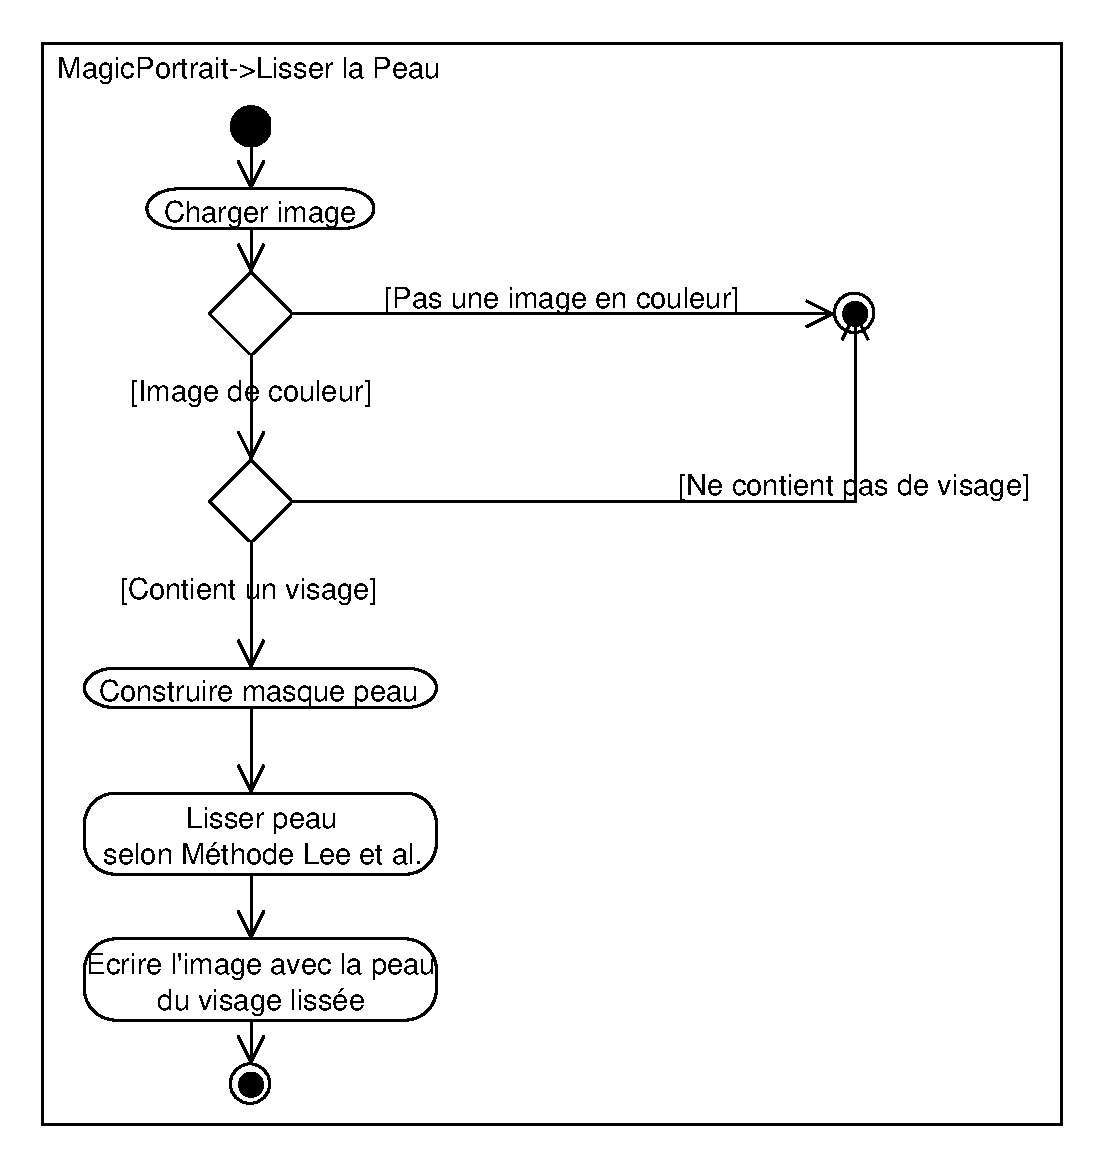
\includegraphics[width=0.5\textwidth]{DiagrammeActivites_10_LissagePeau}
\caption{Fonctionnement du premier module}
\end{figure}
\end{frame}

\begin{frame}{Fonctionnement du module 1: Lissage de la peau}
\begin{figure}
\centering
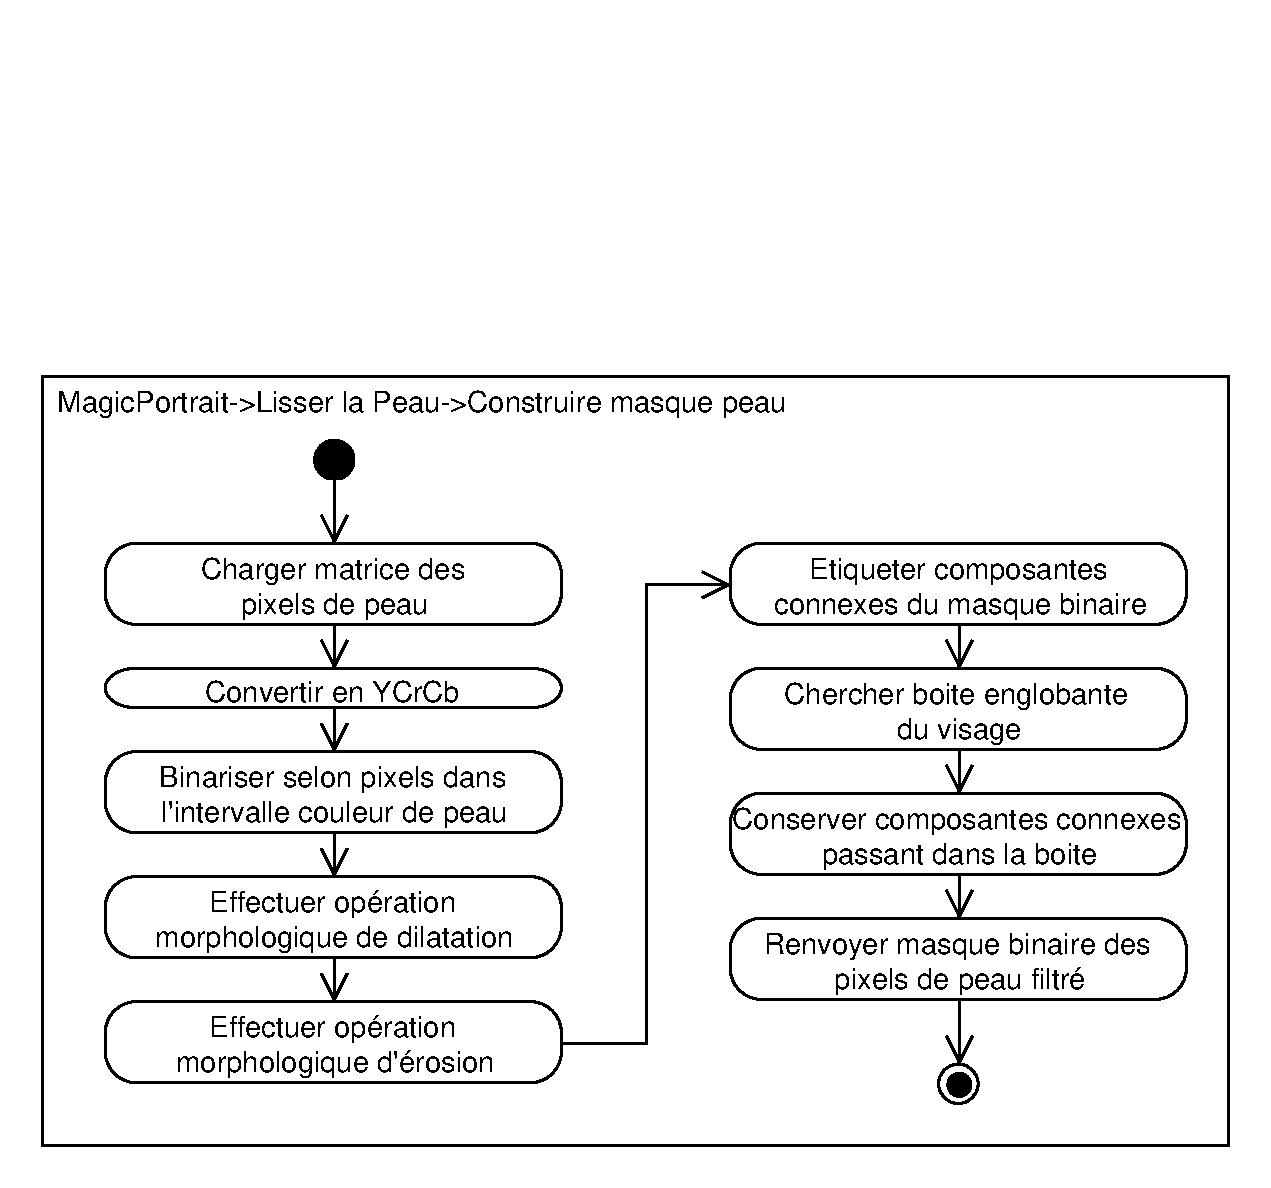
\includegraphics[width=0.6\textwidth]{DiagrammeActivites_11_LissagePeau_Masque}
\caption{Construction du masque des pixels de peau}
\end{figure}
\end{frame}

\begin{frame}{Résultats à l'issue du module 1}
\begin{figure}[htp]
 \centering
 \subfloat[Image originale]{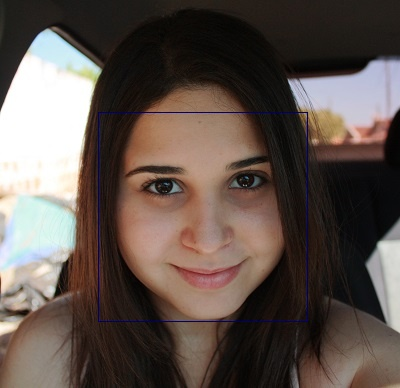
\includegraphics[scale=0.25]{Images/ea_test_lissage_01}}               
 \subfloat[Masque de peau]{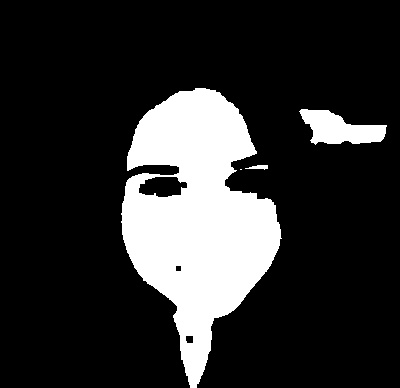
\includegraphics[scale=0.25]{Images/ea_test_lissage_02}}
 \subfloat[Image après lissage]{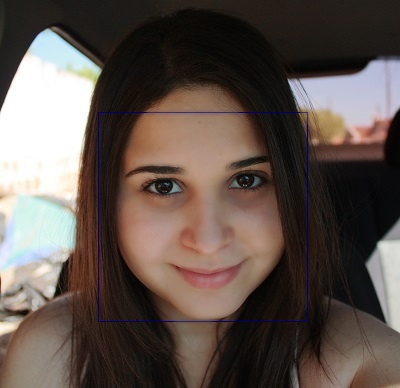
\includegraphics[scale=0.25]{Images/ea_test_lissage_03}}
 \caption{Exemple du lissage de la peau d'un visage avec le premier module}
 \label{fig:lissageExemple}
\end{figure}
\end{frame}

\begin{frame}{Fonctionnement du module 2: Augmentation de la profondeur de champ}
\begin{figure}
\centering
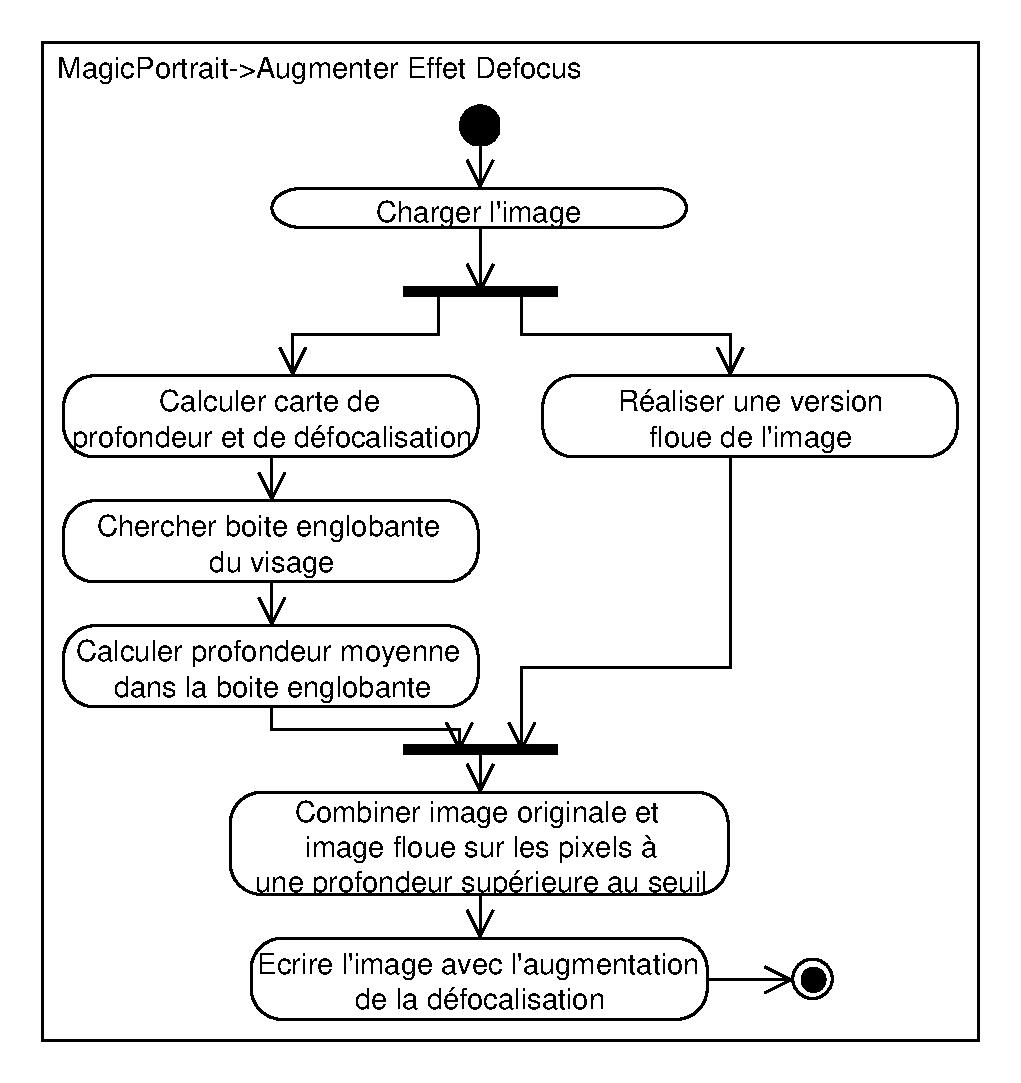
\includegraphics[width=0.4\textwidth]{DiagrammeActivites_20_Profondeur}
\caption{Fonctionnement du deuxième module}
\end{figure}
\end{frame}

\begin{frame}{Résultats à l'issue du module 2}
\begin{figure}[htp]
 \centering
 \subfloat[Image originale]{ \label{fig:ProfExemple1} 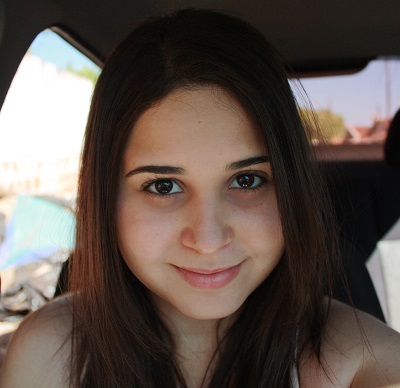
\includegraphics[scale=0.25]{Images/ea_test_prof01}}               
 \subfloat[Pixels au fond]{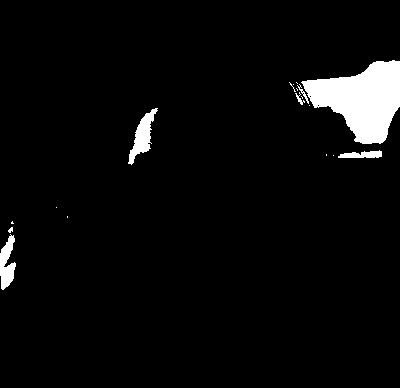
\includegraphics[scale=0.25]{Images/ea_test_prof02}}
 \subfloat[Image après augmentation de la profondeur de champ]{ \label{fig:ProfExemple3}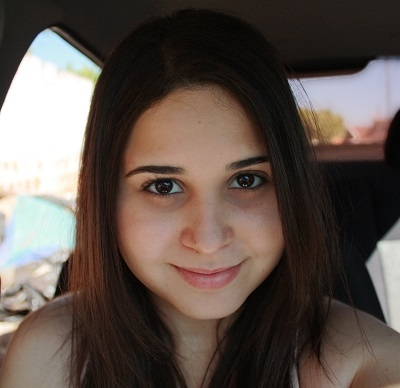
\includegraphics[scale=0.25]{Images/ea_test_prof03}}
 \caption{Exemple de l'augmentation du flou sur les zones en arrière-plan avec le deuxième module}
 \label{fig:ProfExemple}
\end{figure}
\end{frame}

\begin{frame}{Fonctionnement du module 3: Correction du contraste et luminosité}
\begin{figure}
\centering
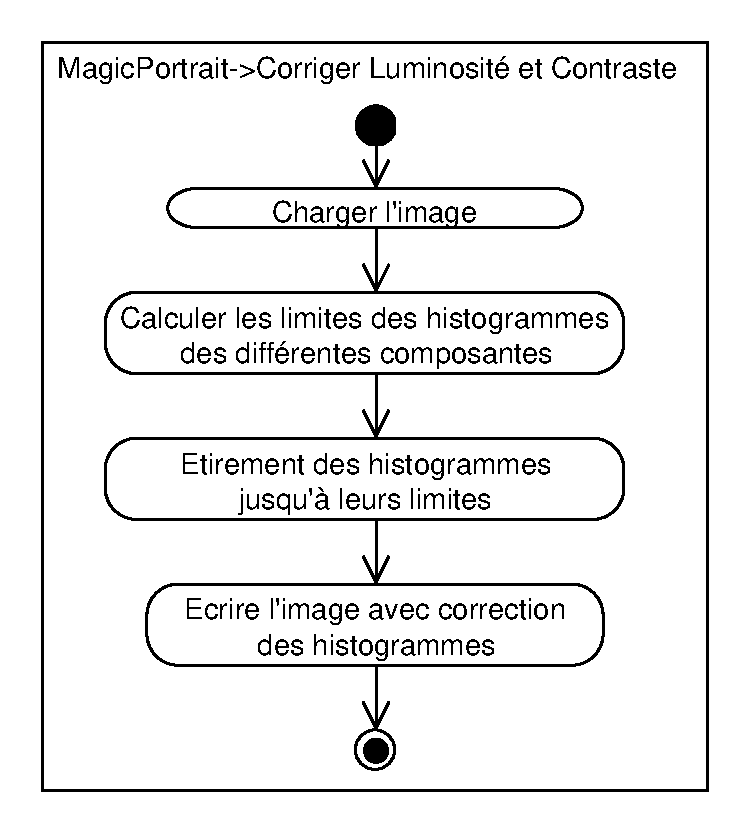
\includegraphics[width=0.5\textwidth]{DiagrammeActivites_30_Contraste}
\caption{Fonctionnement du troisième module}
\end{figure}
\end{frame}

\begin{frame}{Résultats à l'issue du module 3}
\begin{figure}[htp]
 \centering
 \subfloat[Image originale]{ \label{fig:ea_testcontraste01} 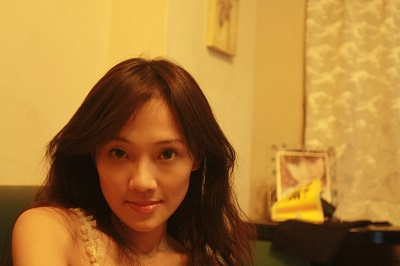
\includegraphics[scale=0.35]{Resultats/pb_avant}}               
 \subfloat[Image plus contrastée]{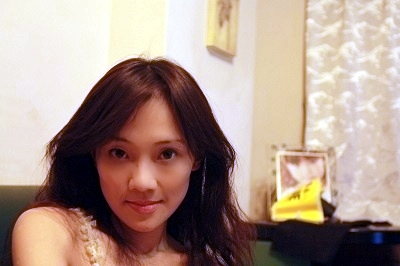
\includegraphics[scale=0.35]{Resultats/pb_apres}}
 \caption{Exemple de correction du contraste et de la luminosité avec le troisième module}
 \label{fig:ContExemple}
\end{figure}
\end{frame}

\subsection{Intégration des modules}

\begin{frame}{Processus d'enchaînement des modules}
\begin{itemize}
\item Création de scripts batchs pour chaque module
\item Pour appliquer un module sur plusieurs images à la fois 
\item Pour effectuer le traitement en une seule fois
\end{itemize}
\end{frame}

%--------------------------------------------------------------------------------------------------------
%Résultats et évaluation---------------------------------------------------------------------------------
%--------------------------------------------------------------------------------------------------------
\section{Résultats et évaluation}

\subsection{Notation de résultats}

\begin{frame}{Présentation de la méthode d'évaluation}
\begin{itemize}
\item Évaluation qualitative et non quantitative
\item Une part de subjectivité
\item Choix d'images de Flickr 
\item "Selfie" et "Portrait" sous licence Creative Commons
\end{itemize}
\pause
\begin{block}{Attribution de trois notes de 1 à 3 sur les résultats : }
Chacune des cibles d'amélioration des modules se voit noter;
\\Plus la note est élevée plus le résultat est satisfaisant.
\end{block}
\end{frame}

\begin{frame}{Quelques exemples}
\begin{table}
\centering
\begin{tabular}{|c|c|c|}	
\hline \textbf{Image avant}  &  \textbf{Image après}  \\ \hline 
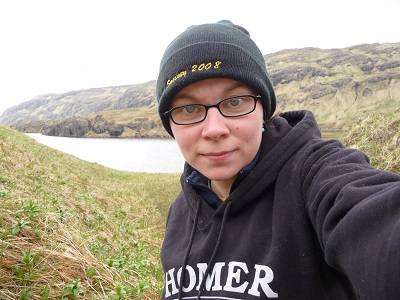
\includegraphics[width=0.45\textwidth]{Resultats/pc_avant} & 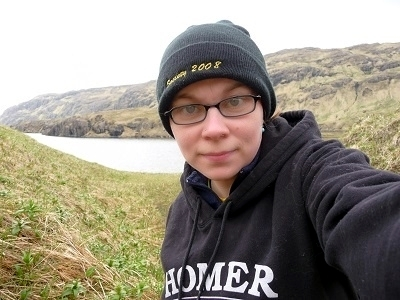
\includegraphics[width=0.45\textwidth]{Resultats/pc_apres} \\ \hline   
\end{tabular}
\caption{Image C à l'issue du traitement développé}
\end{table}

\begin{table}[htbp]
\centering
\begin{tabular}{|c|c|c|}
\hline
Module 1 & Module 2 & Module 3\\ \hline
1 & 1 & 3\\ \hline
\end{tabular}
\caption{Évaluation de l'image C}
\end{table}

\end{frame}

\begin{frame}{Quelques exemples (suite)}
\begin{table}
\centering
\begin{tabular}{|c|c|c|}	
\hline \textbf{Image avant}  &  \textbf{Image après}  \\ \hline 
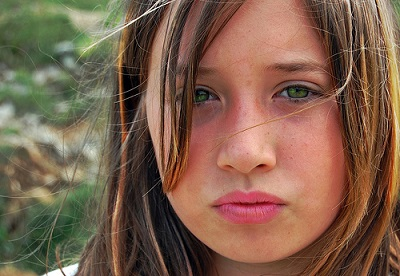
\includegraphics[width=0.45\textwidth]{Resultats/pq_avant} & 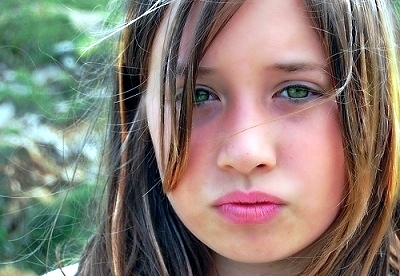
\includegraphics[width=0.45\textwidth]{Resultats/pq_apres} \\ \hline   
\end{tabular}
\caption{Image Q à l'issue du traitement développé}
\end{table}

\begin{table}[htbp]
\centering
\begin{tabular}{|c|c|c|}
\hline
Module 1 & Module 2 & Module 3\\ \hline
3 & 2 & 2\\ \hline
\end{tabular}
\caption{Évaluation de l'image Q}
\end{table}
\end{frame}

\begin{frame}{Quelques exemples (suite bis)}
\begin{table}
\centering
\begin{tabular}{|c|c|c|}	
\hline \textbf{Image avant}  &  \textbf{Image après}  \\ \hline 
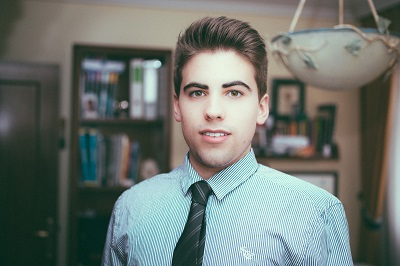
\includegraphics[width=0.45\textwidth]{Resultats/pe_avant} & 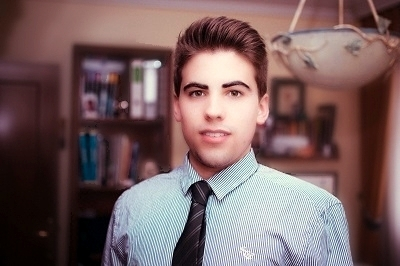
\includegraphics[width=0.45\textwidth]{Resultats/pe_apres} \\ \hline   
\end{tabular}
\caption{Image E à l'issue du traitement développé}
\end{table}

\begin{table}[htbp]
\centering
\begin{tabular}{|c|c|c|}
\hline
Module 1 & Module 2 & Module 3\\ \hline
2 & 3 & 3\\ \hline
\end{tabular}
\caption{Évaluation de l'image E}
\end{table}
\end{frame}

\begin{frame}{Quelques exemples (fin)}
\begin{table}
\centering
\begin{tabular}{|c|c|c|}	
\hline \textbf{Image avant}  &  \textbf{Image après}  \\ \hline 
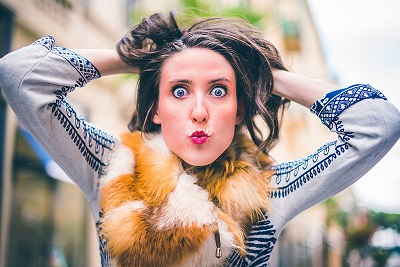
\includegraphics[width=0.45\textwidth]{Resultats/pt_avant} & 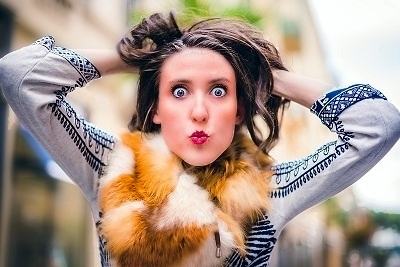
\includegraphics[width=0.45\textwidth]{Resultats/pt_apres} \\ \hline   
\end{tabular}
\caption{Image T à l'issue du traitement développé}
\end{table}

\begin{table}[htbp]
\centering
\begin{tabular}{|c|c|c|}
\hline
Module 1 & Module 2 & Module 3\\ \hline
2 & 3 & 3\\ \hline
\end{tabular}
\caption{Évaluation de l'image T}
\end{table}
\end{frame}

\subsection{Bilan sur les résultats}

\begin{frame}{Évaluation globale}
\begin{itemize}
\item 21 images évaluées
\item Module 1 et 3 plutôt satisfaisants
\item Avis mitigés quant au module d'augmentation de la profondeur de champ
\item Résultats plus intéressants pour les images ayant du flou au départ
\end{itemize}
\end{frame}

%--------------------------------------------------------------------------------------------------------
%Résultats et évaluation---------------------------------------------------------------------------------
%--------------------------------------------------------------------------------------------------------
\section{Évolutions futures}

\subsection{Points à améliorer}

\begin{frame}{Concernant les modules}
\begin{itemize}
\item Construire un masque de peau plus strict
\item Calculer la couleur de la peau dans chaque image
\item Segmenter les composantes de l'image avec les couleurs
\item Changer l'espace couleur pour la correction d'histogramme
\item Temps de calcul à réduire
\end{itemize}
\end{frame}

\subsection{Suggestions de nouvelles pistes}

\begin{frame}{Enchainement global}
\begin{itemize}
\item Revoir l'enchainement des modules
\item Réimplémenter le tout en C++ pour plus d'efficacité
\item Calculer tous les masques à partir de l'image originale
\item Utiliser des méthodes d'apprentissage pour les deux premiers modules
\end{itemize}
\end{frame}

%--------------------------------------------------------------------------------------------------------
%Conclusion----------------------------------------------------------------------------------------------
%--------------------------------------------------------------------------------------------------------
\section{Conclusion}

\begin{frame}{Conclusion}
\begin{itemize}
\item Gain de connaissances concernant le monde de la photographie et de la recherche 
\item Mise en avant de l'importance de la profondeur de champ
\item Plusieurs pistes d'amélioration 
\item Monde de l'amélioration automatique des photographies intéressant pour le grand public
\end{itemize}
\end{frame}

\begin{frame}{Sources}
\begin{itemize}
\item Les articles évoqués et les images utilisées figurent dans la bibliographie du rapport 
\end{itemize}
\end{frame}

\end{document}